\documentclass[11pt,a4paper]{article}

% ─── Packages ────────────────────────────────────────────────────────────────
\usepackage[T1]{fontenc}
\usepackage[utf8]{inputenc}
\usepackage[margin=2.2cm]{geometry}
\usepackage{lmodern}
\usepackage{microtype}
\usepackage{xcolor}
\usepackage{graphicx}
\usepackage{amsmath,amssymb,mathtools}
\usepackage{booktabs}
\usepackage{tabularx}
\usepackage{array}
\usepackage{multirow}
\usepackage{colortbl}
\usepackage{enumitem}
\usepackage{listings}
\usepackage{fancyhdr}
\usepackage{titlesec}
\usepackage{hyperref}
\usepackage{caption}
\usepackage{subcaption}
\usepackage{float}
\usepackage{mdframed}
\usepackage{tcolorbox}
\usepackage{tikz}
\usepackage{pgfplots}
\usepackage{fontawesome5}
\usepackage{setspace}
\usepackage{soul}
\usepackage{parskip}

\usetikzlibrary{shapes.geometric, arrows.meta, positioning, fit,
                decorations.pathreplacing, backgrounds, shadows,
                calc, chains, matrix, shapes.multipart}
\pgfplotsset{compat=1.18}
\tcbuselibrary{skins, breakable, listings}

% ─── Colour Palette ──────────────────────────────────────────────────────────
\definecolor{primary}{HTML}{1A237E}      % deep indigo
\definecolor{accent}{HTML}{283593}       % indigo
\definecolor{highlight}{HTML}{3949AB}    % medium indigo
\definecolor{lightblue}{HTML}{E8EAF6}    % pale indigo bg
\definecolor{darkgray}{HTML}{37474F}
\definecolor{medgray}{HTML}{607D8B}
\definecolor{codebg}{HTML}{F5F5F5}
\definecolor{codeframe}{HTML}{B0BEC5}
\definecolor{nodeblue}{HTML}{1565C0}
\definecolor{nodegreen}{HTML}{2E7D32}
\definecolor{nodeorange}{HTML}{E65100}
\definecolor{nodepurple}{HTML}{6A1B9A}
\definecolor{nodecyan}{HTML}{00695C}
\definecolor{nodered}{HTML}{B71C1C}
\definecolor{rowalt}{HTML}{F0F4FF}
\definecolor{headerrow}{HTML}{1A237E}
\definecolor{warnbg}{HTML}{FFF8E1}
\definecolor{infobg}{HTML}{E3F2FD}

% ─── Hyperref ────────────────────────────────────────────────────────────────
\hypersetup{
  colorlinks=true,
  linkcolor=primary,
  urlcolor=highlight,
  citecolor=highlight,
  pdftitle={Layer10 Memory Graph — Full Architecture Report},
  pdfauthor={Engineering Report},
}

% ─── Section Styles ──────────────────────────────────────────────────────────
\titleformat{\section}
  {\color{primary}\Large\bfseries\sffamily}
  {\color{primary}\thesection.}{0.6em}{}
  [\color{primary}\rule{\linewidth}{1.2pt}\vspace{-4pt}]

\titleformat{\subsection}
  {\color{accent}\large\bfseries\sffamily}
  {\color{accent}\thesubsection}{0.5em}{}

\titleformat{\subsubsection}
  {\color{highlight}\normalsize\bfseries\sffamily}
  {\color{highlight}\thesubsubsection}{0.5em}{}

% ─── Header / Footer ─────────────────────────────────────────────────────────
\pagestyle{fancy}
\fancyhf{}
\fancyhead[L]{\small\sffamily\color{medgray}Layer10 Memory Graph — Architecture Report}
\fancyhead[R]{\small\sffamily\color{medgray}March 6, 2026}
\fancyfoot[C]{\small\sffamily\color{medgray}\thepage}
\renewcommand{\headrulewidth}{0.4pt}
\renewcommand{\headrule}{\hbox to\headwidth{\color{primary}\leaders\hrule height\headrulewidth\hfill}}

% ─── Code Listings ───────────────────────────────────────────────────────────
\lstset{
  backgroundcolor=\color{codebg},
  basicstyle=\ttfamily\footnotesize,
  keywordstyle=\color{primary}\bfseries,
  commentstyle=\color{medgray}\itshape,
  stringstyle=\color{nodeorange},
  numberstyle=\tiny\color{medgray},
  frame=single,
  framesep=4pt,
  rulecolor=\color{codeframe},
  breaklines=true,
  breakatwhitespace=true,
  tabsize=2,
  showstringspaces=false,
  captionpos=b,
}

% ─── tcolorbox styles ─────────────────────────────────────────────────────────
\tcbset{
  boxstyle/.style={
    enhanced, breakable,
    colback=lightblue, colframe=primary,
    fonttitle=\bfseries\sffamily\small,
    boxrule=0.8pt, arc=4pt,
    left=6pt, right=6pt, top=4pt, bottom=4pt,
  },
  mathbox/.style={
    enhanced, breakable,
    colback=white, colframe=highlight,
    fonttitle=\bfseries\sffamily\small,
    boxrule=1pt, arc=3pt,
    left=8pt, right=8pt, top=5pt, bottom=5pt,
    attach boxed title to top left={yshift=-2mm,xshift=6mm},
    boxed title style={colback=highlight, colframe=highlight, arc=2pt, boxrule=0pt},
    title=#1,
  }
}

% ─── Table column helpers ─────────────────────────────────────────────────────
\newcolumntype{L}[1]{>{\raggedright\arraybackslash}p{#1}}
\newcolumntype{C}[1]{>{\centering\arraybackslash}p{#1}}
\newcolumntype{R}[1]{>{\raggedleft\arraybackslash}p{#1}}

% ─── Misc helpers ─────────────────────────────────────────────────────────────
\newcommand{\code}[1]{\texttt{\small#1}}
\newcommand{\term}[1]{\textbf{\textit{#1}}}
\setlength{\parskip}{4pt}
\setlength{\parindent}{0pt}

% ══════════════════════════════════════════════════════════════════════════════
\begin{document}
% ══════════════════════════════════════════════════════════════════════════════

% ─── Title Page ──────────────────────────────────────────────────────────────
\begin{titlepage}
\pagecolor{primary}
\color{white}
\vspace*{2cm}
\begin{center}
  {\fontsize{11}{13}\sffamily\color{white!70!primary} TECHNICAL ARCHITECTURE REPORT}\\[0.6cm]
  {\fontsize{30}{36}\sffamily\bfseries Layer10 Memory Graph}\\[0.3cm]
  {\fontsize{16}{20}\sffamily\color{white!80!primary}
    Enron Email $\rightarrow$ Organisational Knowledge Graph Pipeline}\\[2cm]

  \resizebox{0.92\textwidth}{!}{%
  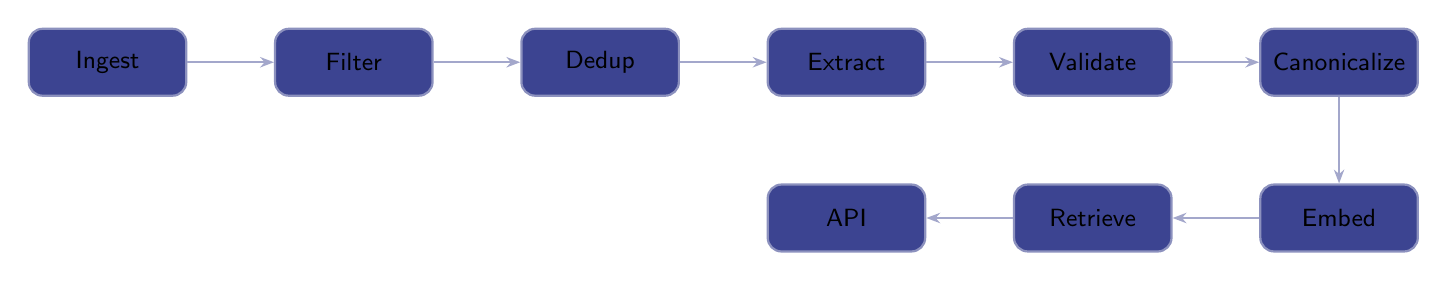
\begin{tikzpicture}[node distance=0.9cm and 1.1cm]
    \tikzstyle{pbox}=[rectangle, rounded corners=5pt, minimum width=2.0cm,
                      minimum height=0.85cm, text centered, font=\small\sffamily,
                      draw=white!50!primary, line width=0.8pt]
    \tikzstyle{arr}=[-{Stealth[length=5pt]}, white!60!primary, line width=0.8pt]

    \node[pbox, fill=white!15!primary] (ing)  {Ingest};
    \node[pbox, fill=white!15!primary, right=of ing] (flt)  {Filter};
    \node[pbox, fill=white!15!primary, right=of flt] (dup)  {Dedup};
    \node[pbox, fill=white!15!primary, right=of dup] (ext)  {Extract};
    \node[pbox, fill=white!15!primary, right=of ext] (val)  {Validate};
    \node[pbox, fill=white!15!primary, right=of val] (can)  {Canonicalize};
    \node[pbox, fill=white!15!primary, below=1.1cm of can] (emb)  {Embed};
    \node[pbox, fill=white!15!primary, left=of emb]  (ret)  {Retrieve};
    \node[pbox, fill=white!15!primary, left=of ret]  (api)  {API};

    \draw[arr] (ing) -- (flt);
    \draw[arr] (flt) -- (dup);
    \draw[arr] (dup) -- (ext);
    \draw[arr] (ext) -- (val);
    \draw[arr] (val) -- (can);
    \draw[arr] (can) -- (emb);
    \draw[arr] (emb) -- (ret);
    \draw[arr] (ret) -- (api);
  \end{tikzpicture}%
  }

  \vfill
  \begin{tabular}{r@{\hspace{0.8em}}l}
    \sffamily\color{white!70!primary}Author:  & \sffamily Shriya Sinha \\[2pt]
    \sffamily\color{white!70!primary}Date:    & \sffamily March 6, 2026 \\[2pt]
    \sffamily\color{white!70!primary}Project: & \sffamily Layer10 Take-Home \\[2pt]
    \sffamily\color{white!70!primary}Dataset: & \sffamily Enron Email Corpus ($\sim$500K messages) \\[2pt]
    \sffamily\color{white!70!primary}Stack:   & \sffamily Python 3.13 · PostgreSQL 16 · pgvector · FastAPI \\
  \end{tabular}
\end{center}
\end{titlepage}
\nopagecolor

% ─── Table of Contents ───────────────────────────────────────────────────────
\tableofcontents
\newpage

% ══════════════════════════════════════════════════════════════════════════════
\section{System Overview}
% ══════════════════════════════════════════════════════════════════════════════

The Layer10 Memory Graph pipeline transforms raw corporate email archives into a
structured, evidence-backed knowledge graph.  Each node is a typed \term{entity}
(Person, Organisation, Project, Topic, Document, Meeting) and each edge is a
\term{claim} — a typed relationship grounded by a verbatim excerpt from the
source email.

\begin{tcolorbox}[boxstyle, title={\faLightbulb\quad Core Design Principle}]
\textbf{Evidence-first:} No claim is stored without a verbatim quote from the
source email that supports it.  This is the single most important quality gate —
it turns the system into a provenance graph, not a hallucination graph.
\end{tcolorbox}

\subsection*{Pipeline at a Glance}

\begin{figure}[H]
\centering
\resizebox{\textwidth}{!}{%
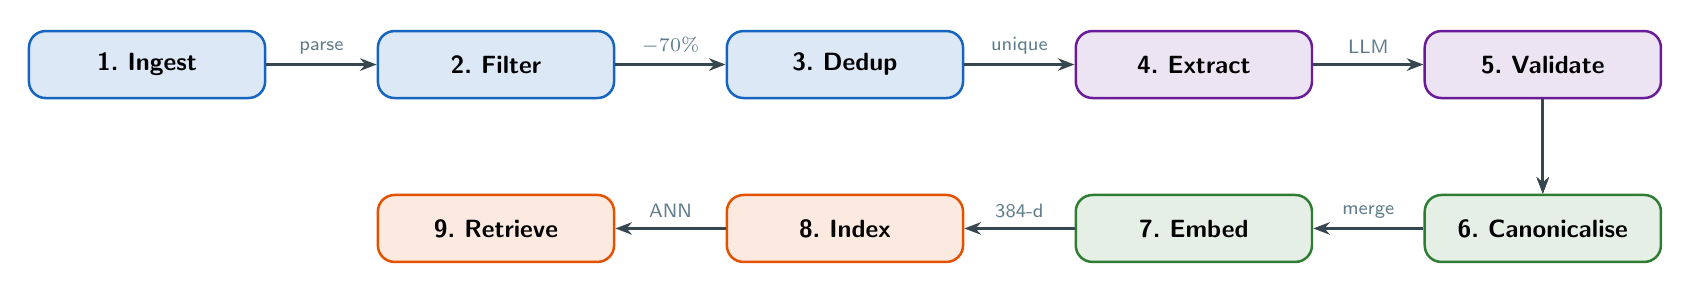
\begin{tikzpicture}[
  node distance=0.55cm and 0.1cm,
  stage/.style={rectangle, rounded corners=6pt, minimum width=3.0cm,
                minimum height=0.85cm, text centered,
                font=\small\sffamily\bfseries, draw, line width=0.9pt},
  arr/.style={-{Stealth[length=6pt]}, darkgray, line width=1pt},
  lbl/.style={font=\scriptsize\sffamily, text=medgray, align=center},
]
  \node[stage, fill=nodeblue!15, draw=nodeblue]   (A) {1.\ Ingest};
  \node[stage, fill=nodeblue!15, draw=nodeblue, right=1.4cm of A] (B) {2.\ Filter};
  \node[stage, fill=nodeblue!15, draw=nodeblue, right=1.4cm of B] (C) {3.\ Dedup};
  \node[stage, fill=nodepurple!12, draw=nodepurple, right=1.4cm of C] (D) {4.\ Extract};
  \node[stage, fill=nodepurple!12, draw=nodepurple, right=1.4cm of D] (E) {5.\ Validate};

  \node[stage, fill=nodegreen!12, draw=nodegreen, below=1.2cm of E] (F) {6.\ Canonicalise};
  \node[stage, fill=nodegreen!12, draw=nodegreen, left=1.4cm of F]  (G) {7.\ Embed};
  \node[stage, fill=nodeorange!12, draw=nodeorange, left=1.4cm of G] (H) {8.\ Index};
  \node[stage, fill=nodeorange!12, draw=nodeorange, left=1.4cm of H] (I) {9.\ Retrieve};

  \draw[arr] (A)--(B) node[lbl,midway,above]{parse};
  \draw[arr] (B)--(C) node[lbl,midway,above]{$-70\%$};
  \draw[arr] (C)--(D) node[lbl,midway,above]{unique};
  \draw[arr] (D)--(E) node[lbl,midway,above]{LLM};
  \draw[arr] (E)--(F);
  \draw[arr] (F)--(G) node[lbl,midway,above]{merge};
  \draw[arr] (G)--(H) node[lbl,midway,above]{384-d};
  \draw[arr] (H)--(I) node[lbl,midway,above]{ANN};

  % vertical connector
  \draw[arr] (E) -- ++(0,-0.55) -| (F);
\end{tikzpicture}%
}
\caption{Nine-stage end-to-end pipeline from raw \texttt{.maildir} files to
  queryable knowledge graph.}
\end{figure}

% ══════════════════════════════════════════════════════════════════════════════
\section{High-Level Architecture}
% ══════════════════════════════════════════════════════════════════════════════

The system is decomposed into three layers that communicate exclusively through
PostgreSQL, so each can be rerun independently.  The \textbf{Ingestion layer}
(blue) parses \texttt{.maildir} files, filters, deduplicates, and threads
emails into \code{raw\_emails}.  The \textbf{Extraction layer} (purple) drives
LLM calls with evidence-grounded validation and writes typed entities and
claims.  The \textbf{Retrieval layer} (orange) embeds entities into 384-d
vectors, indexes them with IVFFlat ANN, and exposes graph queries via FastAPI.


\begin{figure}[H]

\centering
\resizebox{\textwidth}{!}{%
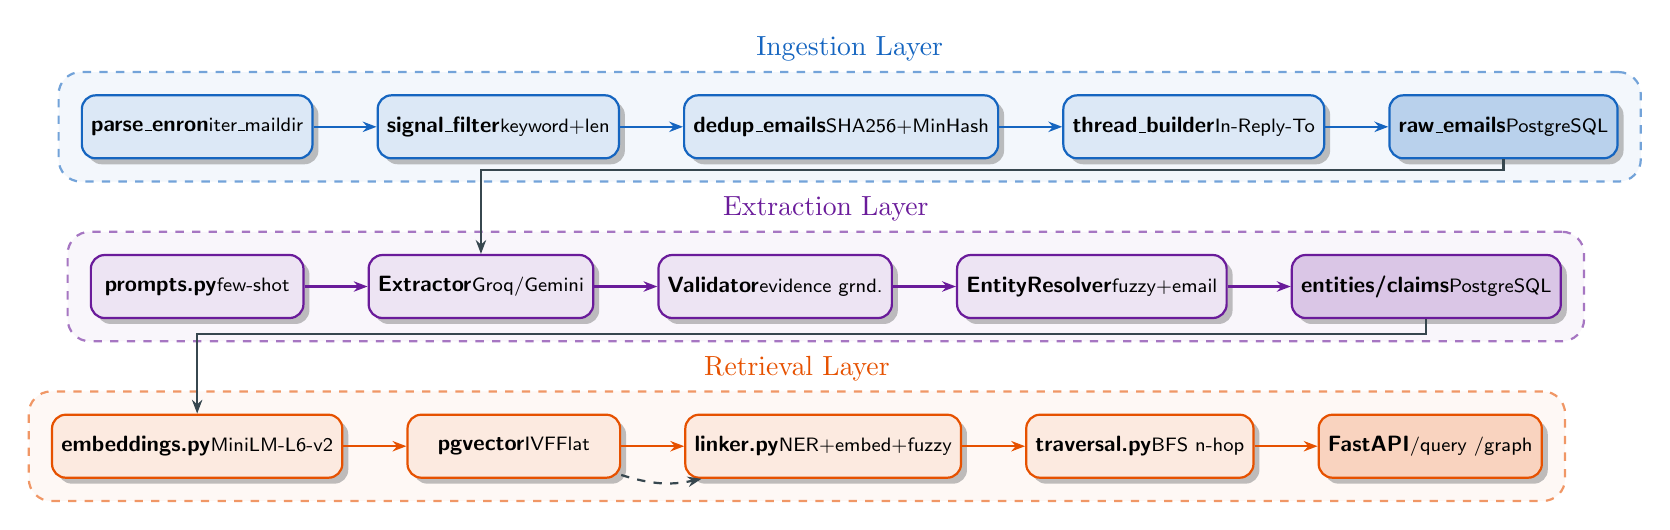
\begin{tikzpicture}[
  mod/.style={rectangle, rounded corners=5pt, minimum width=2.7cm,
              minimum height=0.8cm, text centered,
              font=\footnotesize\sffamily, draw, line width=0.8pt,
              drop shadow},
  grp/.style={rectangle, rounded corners=8pt, draw, dashed, line width=0.8pt,
              inner sep=8pt, font=\small\sffamily\bfseries},
  arr/.style={-{Stealth[length=5pt]}, line width=0.8pt},
  node distance=0.4cm and 0.5cm,
]
  %% Row 1 — Ingestion
  \node[mod, fill=nodeblue!15, draw=nodeblue]   (parse) {\textbf{parse\_enron}\\\scriptsize iter\_maildir};
  \node[mod, fill=nodeblue!15, draw=nodeblue, right=0.8cm of parse] (filt) {\textbf{signal\_filter}\\\scriptsize keyword+len};
  \node[mod, fill=nodeblue!15, draw=nodeblue, right=0.8cm of filt]  (dedup) {\textbf{dedup\_emails}\\\scriptsize SHA256+MinHash};
  \node[mod, fill=nodeblue!15, draw=nodeblue, right=0.8cm of dedup] (thread) {\textbf{thread\_builder}\\\scriptsize In-Reply-To};
  \node[mod, fill=nodeblue!30, draw=nodeblue, right=0.8cm of thread] (rawdb) {\textbf{raw\_emails}\\\scriptsize PostgreSQL};

  \draw[arr,nodeblue] (parse)--(filt);
  \draw[arr,nodeblue] (filt)--(dedup);
  \draw[arr,nodeblue] (dedup)--(thread);
  \draw[arr,nodeblue] (thread)--(rawdb);

  \begin{scope}[on background layer]
    \node[grp, draw=nodeblue!60, fill=nodeblue!5,
          fit=(parse)(filt)(dedup)(thread)(rawdb), label=above:{\color{nodeblue}Ingestion Layer}] {};
  \end{scope}

  %% Row 2 — Extraction
  \node[mod, fill=nodepurple!12, draw=nodepurple, below=1.2cm of parse] (prompt) {\textbf{prompts.py}\\\scriptsize few-shot};
  \node[mod, fill=nodepurple!12, draw=nodepurple, right=0.8cm of prompt] (extr)  {\textbf{Extractor}\\\scriptsize Groq/Gemini};
  \node[mod, fill=nodepurple!12, draw=nodepurple, right=0.8cm of extr]  (valid)  {\textbf{Validator}\\\scriptsize evidence grnd.};
  \node[mod, fill=nodepurple!12, draw=nodepurple, right=0.8cm of valid] (ereso)  {\textbf{EntityResolver}\\\scriptsize fuzzy+email};
  \node[mod, fill=nodepurple!25, draw=nodepurple, right=0.8cm of ereso] (graphdb) {\textbf{entities/claims}\\\scriptsize PostgreSQL};

  \draw[arr,nodepurple] (prompt)--(extr);
  \draw[arr,nodepurple] (extr)--(valid);
  \draw[arr,nodepurple] (valid)--(ereso);
  \draw[arr,nodepurple] (ereso)--(graphdb);
  \draw[arr,darkgray] (rawdb) -- ++(0,-0.55) -| (extr);

  \begin{scope}[on background layer]
    \node[grp, draw=nodepurple!60, fill=nodepurple!4,
          fit=(prompt)(extr)(valid)(ereso)(graphdb), label=above:{\color{nodepurple}Extraction Layer}] {};
  \end{scope}

  %% Row 3 — Retrieval
  \node[mod, fill=nodeorange!12, draw=nodeorange, below=1.2cm of prompt] (emb)  {\textbf{embeddings.py}\\\scriptsize MiniLM-L6-v2};
  \node[mod, fill=nodeorange!12, draw=nodeorange, right=0.8cm of emb]   (pgv)  {\textbf{pgvector}\\\scriptsize IVFFlat};
  \node[mod, fill=nodeorange!12, draw=nodeorange, right=0.8cm of pgv]   (link) {\textbf{linker.py}\\\scriptsize NER+embed+fuzzy};
  \node[mod, fill=nodeorange!12, draw=nodeorange, right=0.8cm of link]  (trav) {\textbf{traversal.py}\\\scriptsize BFS n-hop};
  \node[mod, fill=nodeorange!25, draw=nodeorange, right=0.8cm of trav]  (api)  {\textbf{FastAPI}\\\scriptsize /query /graph};

  \draw[arr,nodeorange] (emb)--(pgv);
  \draw[arr,nodeorange] (pgv)--(link);
  \draw[arr,nodeorange] (link)--(trav);
  \draw[arr,nodeorange] (trav)--(api);
  \draw[arr,darkgray] (graphdb) -- ++(0,-0.6) -| (emb);
  \draw[arr,darkgray,dashed] (pgv) to[bend right=15] (link);

  \begin{scope}[on background layer]
    \node[grp, draw=nodeorange!60, fill=nodeorange!4,
          fit=(emb)(pgv)(link)(trav)(api), label=above:{\color{nodeorange}Retrieval Layer}] {};
  \end{scope}

\end{tikzpicture}%
}
\caption{Full component architecture showing module names, data-flow arrows,
  and layer groupings.  Blue = ingestion, purple = extraction, orange = retrieval.}
\end{figure}
\vspace{-5mm}

\begin{table}[H]
\centering
\small
\begin{tabularx}{\linewidth}{L{3.2cm} X}
\toprule
\rowcolor{headerrow}
\color{white}\textbf{Component} & \color{white}\textbf{Details} \\
\midrule
Database       & PostgreSQL 16 with \code{pgvector}, \code{pg\_trgm}, \code{uuid-ossp} \\
\rowcolor{rowalt}
Runtime        & Python 3.13, fully async (\code{asyncio} + \code{asyncpg}) \\
Schema valid.  & Pydantic v2 — strict types throughout \\
\rowcolor{rowalt}
API            & FastAPI with CORS middleware, Pydantic response models \\
Frontend       & React + Vite + TypeScript (\code{webui/}) \\
\rowcolor{rowalt}
Containerised  & Docker Compose (PostgreSQL + app service) \\
\bottomrule
\end{tabularx}
\end{table}

% ══════════════════════════════════════════════════════════════════════════════
\section{Component Deep Dive}
% ══════════════════════════════════════════════════════════════════════════════

\subsection{Ingestion Layer — \code{ingestion/parse\_enron.py}}

The ingestion layer walks the Enron \texttt{.maildir} directory tree and produces
immutable \code{RawEmail} dataclass instances.

\begin{enumerate}[leftmargin=*, itemsep=2pt]
  \item Open each file with Python's stdlib \code{email} module.
  \item Extract headers: \code{Message-ID}, \code{From}, \code{To/Cc/Bcc},
        \code{Date}, \code{Subject}, \code{In-Reply-To}, \code{References}.
  \item For multipart MIME messages, walk parts and return the first
        \code{text/plain} payload.
  \item Produce a frozen \code{RawEmail} (immutable, \code{\_\_slots\_\_=True}
        for memory efficiency).
\end{enumerate}

Two computed properties drive deduplication:
\begin{align*}
  \texttt{body\_hash} &= \mathrm{SHA\text{-}256}\!\left(\texttt{UTF\text{-}8}(b)\right) \\
  \texttt{dedup\_key} &= \mathrm{SHA\text{-}256}\!\left(\texttt{UTF\text{-}8}\!\left(
      \textit{sender}\,|\,\textit{date}\,|\,\textit{subject}\,|\,\texttt{body\_hash}
    \right)\right)
\end{align*}

A configurable \code{enron\_user\_list} (default: 10 key users) limits scope to
stay within free-tier LLM rate limits.

\subsection{Signal Filter — \code{ingestion/signal\_filter.py}}

A cheap pre-filter running \textbf{before} any LLM call, eliminating $\approx$70\%
of emails.  Three criteria must \emph{all} pass:

\begin{table}[H]
\centering
\small
\begin{tabularx}{\linewidth}{L{2.8cm} X}
\toprule
\rowcolor{headerrow}
\color{white}\textbf{Filter} & \color{white}\textbf{Condition} \\
\midrule
Folder filter  & Folder name must \textbf{not} be in
  \{\code{all\_documents}, \code{deleted\_items}, \code{notes\_inbox},
  \code{contacts}, \code{calendar}, \code{straw}\} \\
\rowcolor{rowalt}
Body length    & $|\texttt{body.strip()}| \geq 50$ characters \\
Keyword signal & At least \textbf{2} of 55 signal keywords appear in
  \code{subject + body} (case-insensitive) \\
\bottomrule
\end{tabularx}
\caption{Signal filter criteria.  All three must pass for an email to advance.}
\end{table}

The 55-term keyword list covers: key Enron executives (\textit{skilling, lay,
fastow}), named entities (\textit{LJM, Raptor, Azurix}), financial signals
(\textit{mark-to-market, 10-k, restatement}), decision verbs (\textit{approved,
resigned}), and risk terms (\textit{write-down, collateral}).

\subsection{Email Deduplication — \code{ingestion/dedup\_emails.py}}

Three-level deduplication with a fully auditable \code{DedupEvent} trail:

\begin{figure}[H]
\centering
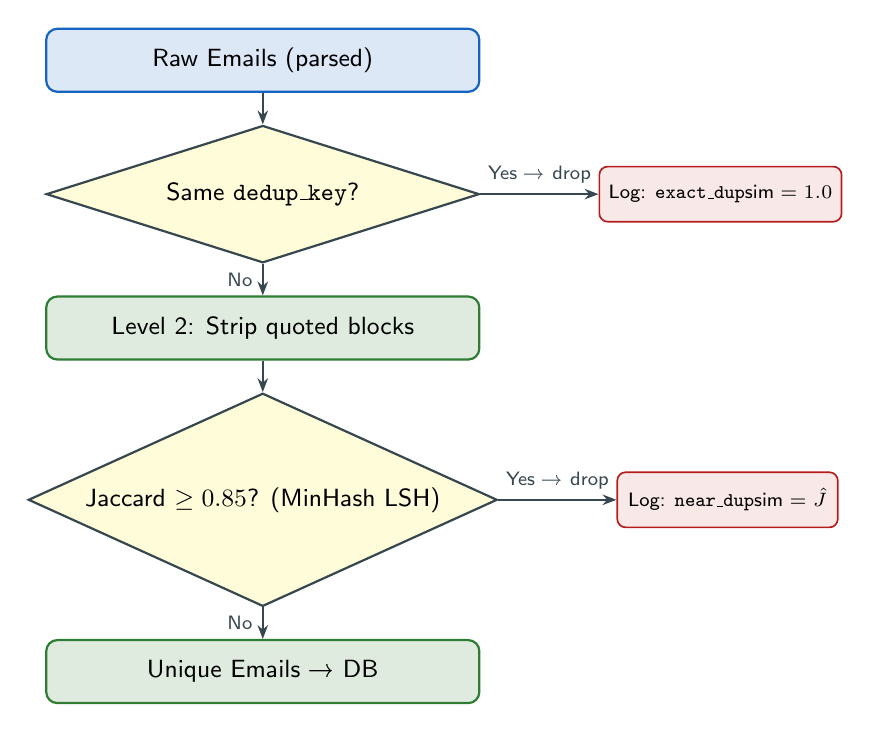
\begin{tikzpicture}[
  node distance=0.5cm,
  box/.style={rectangle, rounded corners=4pt, minimum width=5.5cm,
              minimum height=0.8cm, text centered,
              font=\small\sffamily, draw, line width=0.8pt},
  dec/.style={diamond, aspect=2.2, minimum width=5.5cm, minimum height=0.9cm,
              text centered, font=\small\sffamily, draw, line width=0.8pt},
  arr/.style={-{Stealth[length=5pt]}, darkgray, line width=0.9pt},
  side/.style={rectangle, rounded corners=3pt, minimum width=2.8cm,
               minimum height=0.7cm, text centered,
               font=\scriptsize\sffamily, draw, line width=0.6pt,
               fill=nodered!10, draw=nodered},
]
  \node[box, fill=nodeblue!15, draw=nodeblue] (in)   {Raw Emails (parsed)};
  \node[dec, fill=yellow!15,   draw=darkgray, below=0.4cm of in]  (d1)   {Same \texttt{dedup\_key}?};
  \node[box, fill=nodegreen!15, draw=nodegreen, below=0.4cm of d1] (qs)   {Level 2: Strip quoted blocks};
  \node[dec, fill=yellow!15,   draw=darkgray, below=0.4cm of qs]  (d2)   {Jaccard $\geq 0.85$? (MinHash LSH)};
  \node[box, fill=nodegreen!15, draw=nodegreen, below=0.4cm of d2] (out)  {Unique Emails → DB};

  \node[side, right=1.5cm of d1] (drop1) {Log: \texttt{exact\_dup}\\$\text{sim}=1.0$};
  \node[side, right=1.5cm of d2] (drop2) {Log: \texttt{near\_dup}\\$\text{sim}=\hat{J}$};


  \draw[arr] (in)  -- (d1);
  \draw[arr] (d1)  -- node[left,font=\scriptsize\sffamily]{No} (qs);
  \draw[arr] (qs)  -- (d2);
  \draw[arr] (d2)  -- node[left,font=\scriptsize\sffamily]{No} (out);
  \draw[arr] (d1)  -- node[above,font=\scriptsize\sffamily]{Yes → drop} (drop1);
  \draw[arr] (d2)  -- node[above,font=\scriptsize\sffamily]{Yes → drop} (drop2);
\end{tikzpicture}
\caption{Three-level deduplication flowchart.  Every dropped email is logged
  with its canonical ID, reason, and similarity score.}
\end{figure}

\subsection{LLM Extraction Engine — \code{extraction/extractor.py}}

The extraction engine converts email text to structured entities and claims:

\begin{figure}[H]
\centering
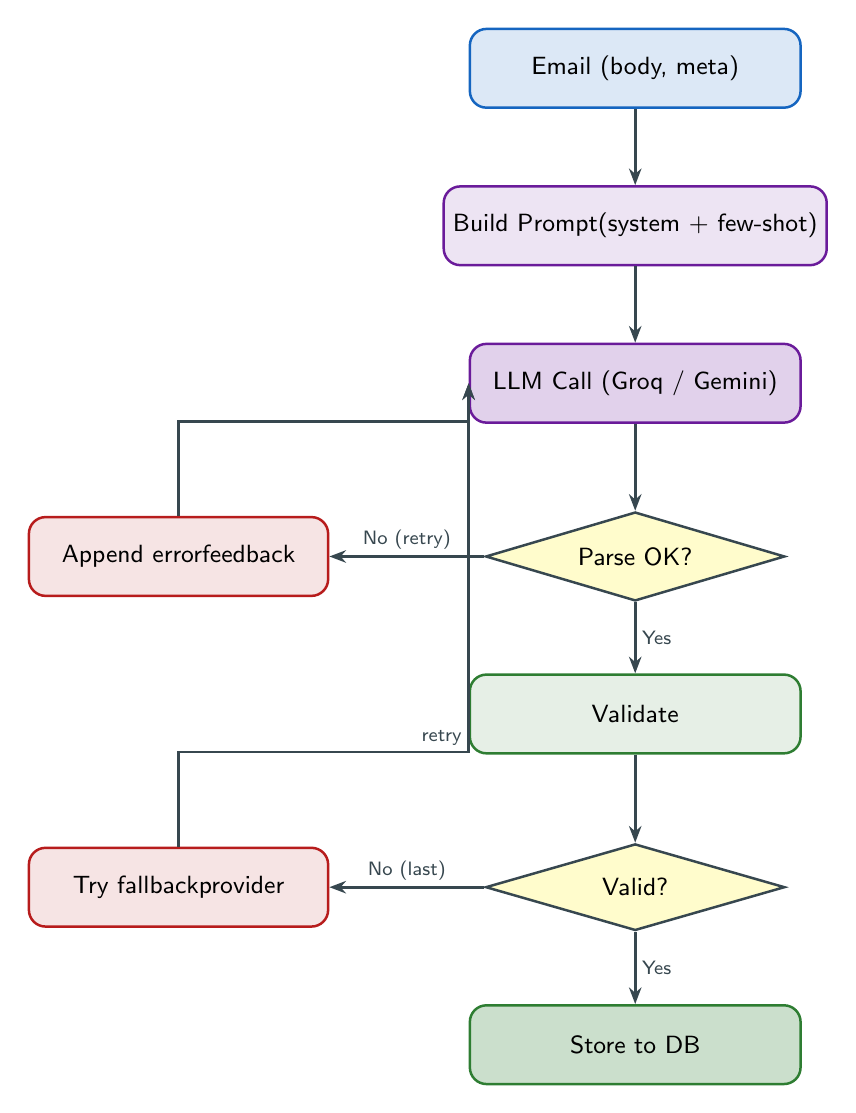
\begin{tikzpicture}[
  box/.style={rectangle, rounded corners=6pt, minimum width=4.2cm,
              minimum height=1.0cm, text centered,
              font=\small\sffamily, draw, line width=0.9pt},
  dec/.style={diamond, aspect=2.5, minimum width=3.8cm, minimum height=1.1cm,
              text centered, font=\small\sffamily, draw, line width=0.9pt},
  side/.style={rectangle, rounded corners=6pt, minimum width=3.8cm,
               minimum height=1.0cm, text centered,
               font=\small\sffamily, draw, line width=0.9pt},
  arr/.style={-{Stealth[length=6pt]}, darkgray, line width=1.0pt},
  lbl/.style={font=\scriptsize\sffamily, fill=white, inner sep=2pt},
]
  %% ── Main vertical spine (centre column, x=0) ────────────────────────────
  \node[box,  fill=nodeblue!15,   draw=nodeblue]   (em)  at (0,  0)    {Email (body, meta)};
  \node[box,  fill=nodepurple!12, draw=nodepurple] (pm)  at (0, -2.0)  {Build Prompt\\(system + few-shot)};
  \node[box,  fill=nodepurple!20, draw=nodepurple] (llm) at (0, -4.0)  {LLM Call (Groq / Gemini)};
  \node[dec,  fill=yellow!20,     draw=darkgray]   (pok) at (0, -6.2)  {Parse OK?};
  \node[box,  fill=nodegreen!12,  draw=nodegreen]  (val) at (0, -8.2)  {Validate};
  \node[dec,  fill=yellow!20,     draw=darkgray]   (vok) at (0,-10.4)  {Valid?};
  \node[box,  fill=nodegreen!25,  draw=nodegreen]  (st)  at (0,-12.4)  {Store to DB};

  %% ── Feedback boxes (left column, x=-5.8) ────────────────────────────────
  \node[side, fill=nodered!12, draw=nodered]  (fb)   at (-5.8, -6.2)  {Append error\\feedback};
  \node[side, fill=nodered!12, draw=nodered]  (fall) at (-5.8,-10.4)  {Try fallback\\provider};

  %% ── Main-flow arrows ─────────────────────────────────────────────────────
  \draw[arr] (em)  -- (pm);
  \draw[arr] (pm)  -- (llm);
  \draw[arr] (llm) -- (pok);
  \draw[arr] (pok) -- node[lbl, right]{Yes} (val);
  \draw[arr] (val) -- (vok);
  \draw[arr] (vok) -- node[lbl, right]{Yes} (st);

  %% ── "No (retry)" path: pok → fb → llm ───────────────────────────────────
  \draw[arr] (pok.west) -- node[lbl, above]{No (retry)} (fb.east);
  \draw[arr] (fb.north) -- ++(0, 1.2) -| (llm.west);

  %% ── "No (last)" path: vok → fall → pm ───────────────────────────────────
  \draw[arr] (vok.west) -- node[lbl, above]{No (last)} (fall.east);
  \draw[arr] (fall.north) -- ++(0, 1.2) -| node[lbl, above left]{retry} (llm.west);

\end{tikzpicture}
\caption{LLM extraction retry loop with self-correction feedback and fallback
  provider.}
\end{figure}

\textbf{Key configuration:} temperature $= 0.1$; rate limit $= 80$ RPM
(\code{aiolimiter}); concurrency $= 20$ tasks (\code{asyncio.Semaphore});
max retries $= 3$.

\subsection{Extraction Validator — \code{extraction/validator.py}}

\begin{figure}[H]
\centering
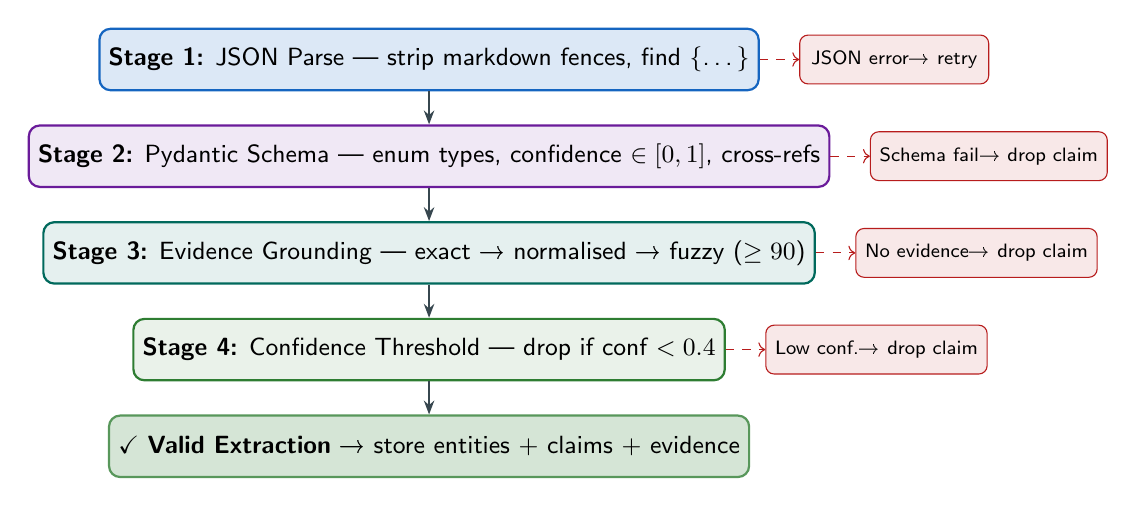
\begin{tikzpicture}[
  st/.style={rectangle, rounded corners=4pt, minimum width=7cm,
             minimum height=0.78cm, text centered,
             font=\small\sffamily, draw, line width=0.8pt},
  arr/.style={-{Stealth[length=5pt]}, darkgray, line width=0.9pt},
  node distance=0.42cm,
  drop/.style={rectangle, rounded corners=3pt, minimum width=2.4cm,
               minimum height=0.62cm, text centered,
               font=\scriptsize\sffamily, fill=nodered!10, draw=nodered},
]
  \node[st, fill=nodeblue!15, draw=nodeblue]      (s1) {\textbf{Stage 1:} JSON Parse — strip markdown fences, find \{\ldots\}};
  \node[st, fill=nodepurple!10, draw=nodepurple, below=of s1] (s2) {\textbf{Stage 2:} Pydantic Schema — enum types, confidence $\in[0,1]$, cross-refs};
  \node[st, fill=nodecyan!10, draw=nodecyan, below=of s2]     (s3) {\textbf{Stage 3:} Evidence Grounding — exact → normalised → fuzzy ($\geq 90$)};
  \node[st, fill=nodegreen!10, draw=nodegreen, below=of s3]   (s4) {\textbf{Stage 4:} Confidence Threshold — drop if conf $< 0.4$};
  \node[st, fill=nodegreen!20, draw=nodegreen!80, below=of s4](s5) {$\checkmark$ \textbf{Valid Extraction} → store entities + claims + evidence};

  \draw[arr] (s1)--(s2);
  \draw[arr] (s2)--(s3);
  \draw[arr] (s3)--(s4);
  \draw[arr] (s4)--(s5);

  \node[drop, right=0.5cm of s1] (d1) {JSON error\\→ retry};
  \node[drop, right=0.5cm of s2] (d2) {Schema fail\\→ drop claim};
  \node[drop, right=0.5cm of s3] (d3) {No evidence\\→ drop claim};
  \node[drop, right=0.5cm of s4] (d4) {Low conf.\\→ drop claim};

  \draw[->, nodered, dashed] (s1.east) -- (d1.west);
  \draw[->, nodered, dashed] (s2.east) -- (d2.west);
  \draw[->, nodered, dashed] (s3.east) -- (d3.west);
  \draw[->, nodered, dashed] (s4.east) -- (d4.west);
\end{tikzpicture}
\caption{Four-stage validation pipeline.  Each stage can drop individual claims;
  only failures at stage 1 trigger a full retry.}
\end{figure}

\subsection{Entity Resolver — \code{dedup/entity\_resolver.py}}

Resolves multiple surface forms of the same real-world entity into a single
canonical record via greedy two-pass clustering:

\begin{enumerate}[leftmargin=*, itemsep=3pt]
  \item \textbf{Pass 1 — Email Address Clustering} (confidence 0.95): entities
    sharing an email address in their alias set are merged.  Longest canonical
    name becomes representative.
  \item \textbf{Pass 2 — Fuzzy Name Matching} (confidence $= \hat{s}$): all
    pairs within the same entity type are scored; pairs with
    $\hat{s} \geq 0.82$ are merged greedily, highest scores first.
\end{enumerate}

Every merge is a transitive \code{absorb} operation: all aliases, email
addresses, and properties are folded into the canonical entity.  A
\code{MergeEvent} audit record (with \code{reversed\_at} support) is written
for every merge.

\subsection{Storage Layer — PostgreSQL 16 + pgvector}

\begin{table}[H]
\centering
\small
\begin{tabularx}{\linewidth}{L{3.2cm} L{2.8cm} X}
\toprule
\rowcolor{headerrow}
\color{white}\textbf{Table} & \color{white}\textbf{Primary Key} & \color{white}\textbf{Purpose} \\
\midrule
\code{raw\_emails}         & \code{message\_id} TEXT & Parsed email storage; indexed by \code{dedup\_key} \\
\rowcolor{rowalt}
\code{email\_threads}      & \code{thread\_id} TEXT  & Conversation thread groups \\
\code{email\_dedup\_log}   & UUID               & Artifact dedup audit trail \\
\rowcolor{rowalt}
\code{entities}            & UUID               & Graph nodes — canonical entities + JSONB properties \\
\code{claims}              & UUID               & Graph edges — typed relationships + temporal windows \\
\rowcolor{rowalt}
\code{evidence}            & UUID               & Evidence pointers: claim $\to$ source excerpt \\
\code{entity\_embeddings}  & entity\_id UUID FK & 384-dim vectors (pgvector) \\
\rowcolor{rowalt}
\code{claim\_embeddings}   & claim\_id UUID FK  & 384-dim vectors (pgvector) \\
\code{processing\_log}     & UUID, UNIQUE(email\_id, version) & Idempotency gate \\
\rowcolor{rowalt}
\code{merge\_events}       & UUID               & Entity/claim merge audit with reversal support \\
\bottomrule
\end{tabularx}
\caption{10-table PostgreSQL schema.  Temporal validity columns on
  \code{claims} support bitemporal queries.}
\end{table}

\subsection{Retrieval API — \code{retrieval/api.py}}

The main \code{GET /api/query?q=\ldots} endpoint runs a three-stage pipeline:

\begin{enumerate}[leftmargin=*, itemsep=3pt]
  \item \textbf{Entity Linking} (\code{linker.py}): four strategies —
    regex NER, fuzzy trigram match (\code{pg\_trgm}), embedding cosine ANN,
    fallback word search.
  \item \textbf{Graph Expansion} (\code{traversal.py}): BFS from seed entities
    up to \code{depth} hops; per-type diversity cap of 5 claims.
  \item \textbf{Context Pack Assembly} (\code{context\_pack.py}): structured
    response with entity summaries, claims, and verbatim evidence snippets.
\end{enumerate}

% ══════════════════════════════════════════════════════════════════════════════
\section{Data Models \& Ontology}
% ══════════════════════════════════════════════════════════════════════════════

\subsection{Entity Types (Graph Nodes)}

\begin{table}[H]
\centering\small
\begin{tabularx}{\linewidth}{L{2.6cm} L{3.2cm} X}
\toprule
\rowcolor{headerrow}
\color{white}\textbf{Type} & \color{white}\textbf{Example} & \color{white}\textbf{Rationale} \\
\midrule
\textbf{Person}       & Kenneth Lay, Jeff Skilling & Central nodes — most claims flow through people \\
\rowcolor{rowalt}
\textbf{Organization} & Enron Corp, McKinsey & Internal \& external institutions \\
\textbf{Project}      & California Energy Deal & Named initiatives referenced in emails \\
\rowcolor{rowalt}
\textbf{Topic}        & Risk Management & Abstract themes for topical clustering \\
\textbf{Document}     & Q3 Report & Referenced artefacts (reports, agreements) \\
\rowcolor{rowalt}
\textbf{Meeting}      & Board Meeting Jan 14 & Scheduled events mentioned in emails \\
\bottomrule
\end{tabularx}
\end{table}

\subsection{Claim Types (Graph Edges)}

\begin{figure}[H]
\centering
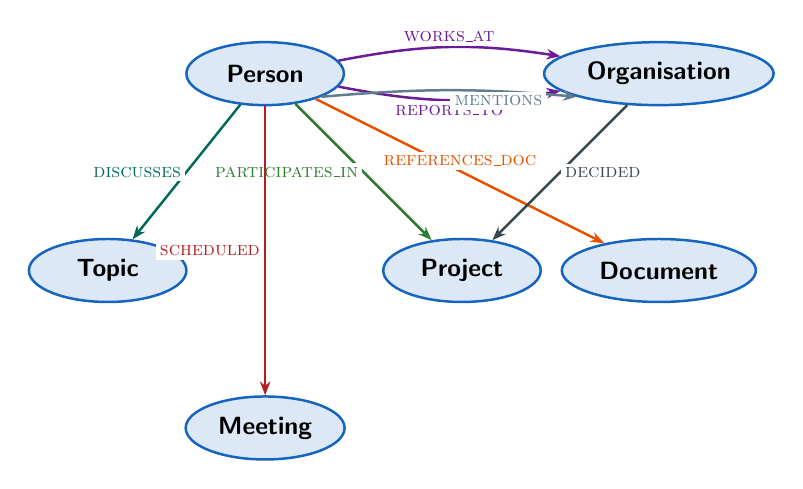
\begin{tikzpicture}[
  ent/.style={ellipse, minimum width=2.0cm, minimum height=0.8cm,
              text centered, font=\small\sffamily\bfseries,
              draw, line width=0.9pt, fill=nodeblue!15, draw=nodeblue},
  rel/.style={-{Stealth[length=5pt]}, line width=0.9pt},
  lbl/.style={font=\scriptsize\sffamily, fill=white, inner sep=1.5pt},
]
  \node[ent] (ken)  at (0,0)     {Person};
  \node[ent] (org)  at (5,0)     {Organisation};
  \node[ent] (proj) at (2.5,-2.5){Project};
  \node[ent] (top)  at (-2,-2.5) {Topic};
  \node[ent] (doc)  at (5,-2.5)  {Document};
  \node[ent] (meet) at (0,-4.5)  {Meeting};

  \draw[rel, nodepurple]  (ken)  to[bend left=10]  node[lbl,above]{\textsc{works\_at}} (org);
  \draw[rel, nodepurple]  (ken)  to[bend right=10] node[lbl,below]{\textsc{reports\_to}} (org);
  \draw[rel, nodegreen]   (ken)  -- node[lbl,left] {\textsc{participates\_in}} (proj);
  \draw[rel, nodecyan]    (ken)  -- node[lbl,left] {\textsc{discusses}} (top);
  \draw[rel, nodeorange]  (ken)  -- node[lbl,above]{\textsc{references\_doc}} (doc);
  \draw[rel, nodered]     (ken)  -- node[lbl,left] {\textsc{scheduled}} (meet);
  \draw[rel, darkgray]    (org)  -- node[lbl,right]{\textsc{decided}} (proj);
  \draw[rel, medgray]     (ken.south east) to[bend left=5] node[lbl,below right]{\textsc{mentions}} (org.south west);
\end{tikzpicture}
\caption{Nine claim types as typed edges between entity nodes.}
\end{figure}

% ══════════════════════════════════════════════════════════════════════════════
\section{Mathematics \& Algorithms}
% ══════════════════════════════════════════════════════════════════════════════

\subsection{SHA-256 Exact Deduplication}

\begin{tcolorbox}[mathbox={SHA-256 Dedup Keys}]
\begin{align}
  \texttt{body\_hash} &= \mathrm{SHA\text{-}256}\!\bigl(\texttt{UTF-8}(\text{body})\bigr)
    \quad \text{[256 bits, 64 hex chars]} \\[4pt]
  \texttt{dedup\_key} &= \mathrm{SHA\text{-}256}\!\Bigl(\texttt{UTF-8}\bigl(
    \underbrace{\text{sender} \mathbin{|} \text{date} \mathbin{|} \text{subject}
    \mathbin{|} \texttt{body\_hash}}_{\text{composite key fields}}
  \bigr)\Bigr)
\end{align}
Collision probability for $n = 5\times10^5$ emails:
$\;P(\text{collision}) \approx \dfrac{n^2}{2^{257}} \approx 0.$
\end{tcolorbox}

Exact dedup is $\mathcal{O}(n)$: one hash computation and one set lookup per email.

\subsection{MinHash \& Jaccard Similarity (Near-Dedup)}

\subsubsection*{Jaccard Similarity}

For two email bodies $A$, $B$ represented as sets of character $k$-shingles
($k=5$):
\begin{equation}
  J(A,B) = \frac{|A \cap B|}{|A \cup B|} \in [0,1]
\end{equation}
Threshold: $J(A,B) \geq 0.85 \Rightarrow$ near-duplicate.
Brute-force computation over $n$ emails requires $\mathcal{O}(n^2)$ pairs —
infeasible at scale.

\subsubsection*{MinHash Approximation}

For $p=128$ independent hash permutations $\{h_i\}$:
\begin{equation}
  \text{sig}(A)[i] = \min_{s \in \text{shingles}(A)} h_i(s)
\end{equation}

The fundamental MinHash property:
\begin{equation}
  \Pr\!\bigl[\,\text{sig}(A)[i] = \text{sig}(B)[i]\,\bigr] = J(A,B)
\end{equation}

The unbiased estimator of Jaccard:
\begin{equation}
  \hat{J}(A,B) = \frac{1}{p}\sum_{i=1}^{p} \mathbf{1}\!\bigl[\text{sig}(A)[i] = \text{sig}(B)[i]\bigr]
\end{equation}

Estimation error with $p=128$:
\begin{equation}
  \sigma\!\bigl[\hat{J}(A,B)\bigr] = \sqrt{\frac{J(1-J)}{p}} \;\leq\;
  \frac{1}{2\sqrt{128}} \approx 0.044
\end{equation}

\subsubsection*{LSH Banding for Sub-linear Search}

The signature is split into $b$ bands of $r$ rows each ($b \cdot r = 128$).
Two emails become a \emph{candidate pair} if they collide in $\geq 1$ band:
\begin{equation}
  P(\text{candidate pair}) = 1 - \bigl(1 - J^r\bigr)^b
\end{equation}

The S-curve inflection (effective threshold):
\begin{equation}
  t \approx \left(\frac{1}{b}\right)^{1/r}
\end{equation}

\begin{figure}[H]
\centering
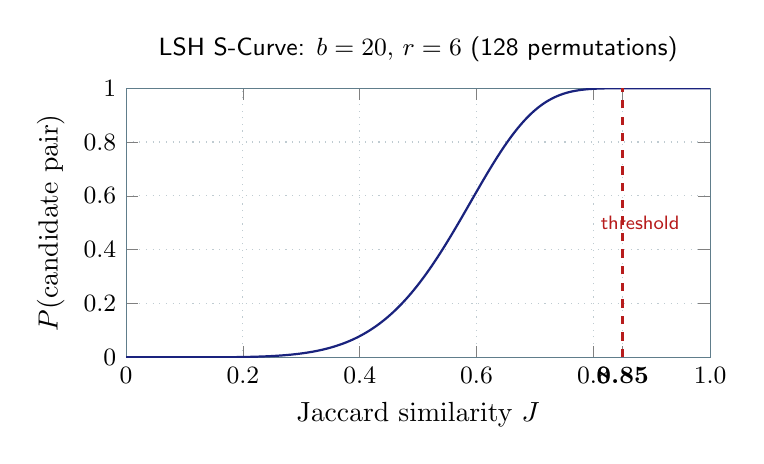
\begin{tikzpicture}
\begin{axis}[
  width=9cm, height=5cm,
  xlabel={Jaccard similarity $J$},
  ylabel={$P(\text{candidate pair})$},
  xmin=0, xmax=1, ymin=0, ymax=1,
  grid=major, grid style={dotted, medgray!40},
  xtick={0,0.2,0.4,0.6,0.8,0.85,1.0},
  xticklabels={0,0.2,0.4,0.6,0.8,\textbf{0.85},1.0},
  ytick={0,0.2,0.4,0.6,0.8,1.0},
  tick label style={font=\small},
  axis line style={medgray},
  title style={font=\small\sffamily},
  title={LSH S-Curve: $b=20,\,r=6$ (128 permutations)},
]
  \addplot[thick, primary, domain=0:1, samples=200]
    {1 - (1 - x^6)^20};
  \addplot[dashed, nodered, very thick] coordinates {(0.85,0) (0.85,1)};
  \node[font=\scriptsize\sffamily, text=nodered] at (axis cs:0.88,0.5)
    {threshold};
\end{axis}
\end{tikzpicture}
\caption{LSH S-curve showing the sharp transition near the 0.85 Jaccard
  threshold.  Pairs above this line are likely candidates.}
\end{figure}

\subsection{Name Similarity Scoring}

A weighted composite of three signals drives entity resolution:
\begin{equation}
  \boxed{\hat{s}(A,B) = 0.4\cdot r_\text{full}(A,B)
                       + 0.3\cdot s_\text{last}(A,B)
                       + 0.3\cdot s_\text{first}(A,B)}
\end{equation}

where $r_\text{full}$ is the normalised Levenshtein ratio:
\begin{equation}
  r_\text{full}(A,B)
    = 1 - \frac{\mathrm{edit\_distance}(A,B)}{\max(|A|,|B|)}
\end{equation}

and the component scores are:
\begin{align}
  s_\text{last}(A,B) &= \begin{cases}
    1.0 & \text{if } \text{last}_A = \text{last}_B \\
    r(\text{last}_A, \text{last}_B) & \text{otherwise}
  \end{cases} \\[6pt]
  s_\text{first}(A,B) &= \begin{cases}
    0.9 & \text{if one first name is a prefix of the other (nickname)} \\
    r(\text{first}_A, \text{first}_B) & \text{otherwise}
  \end{cases}
\end{align}

\textbf{Worked example — ``Ken Lay'' vs.\ ``Kenneth Lay'':}
\begin{center}
\small
\begin{tabular}{lcc}
\toprule
\textbf{Signal} & \textbf{Raw score} & \textbf{Weighted} \\
\midrule
$r_\text{full}$: $1 - 3/\max(7,11) = 0.73$ & 0.73 & $0.4 \times 0.73 = 0.29$ \\
$s_\text{last}$: ``lay'' $=$ ``lay'' (exact) & 1.00 & $0.3 \times 1.00 = 0.30$ \\
$s_\text{first}$: ``ken'' prefix of ``kenneth'' & 0.90 & $0.3 \times 0.90 = 0.27$ \\
\midrule
\multicolumn{2}{r}{\textbf{Total $\hat{s}$}} & \textbf{0.86} $\geq 0.82$ \checkmark \\
\bottomrule
\end{tabular}
\end{center}

\subsection{Evidence Verification (Fuzzy Partial Matching)}

\begin{tcolorbox}[mathbox={Evidence Grounding Algorithm}]
\textbf{Input:} excerpt $e$, email body $b$\\[4pt]
\textbf{Step 1 — Exact:}  $\texttt{b.find}(e) \neq -1 \Rightarrow$ \textbf{accept}\\
\textbf{Step 2 — Normalised:}  $\texttt{normalise}(e) \in \texttt{normalise}(b) \Rightarrow$ \textbf{accept}\\
\textbf{Step 3 — Fuzzy:}
\[
  \texttt{partial\_ratio}(e, b)
  = \max_{\substack{S \subseteq b \\ |S|=|e|}} \texttt{ratio}(e, S) \geq 90 \Rightarrow \textbf{accept}
\]
\textbf{Otherwise:} claim is \textbf{dropped} (hallucinated excerpt)
\end{tcolorbox}

The 90\% fuzzy threshold tolerates minor LLM transcription errors (whitespace
normalisation, Unicode variants) while rejecting fabricated excerpts.

\subsection{Vector Embeddings \& Cosine Similarity}

Entity and claim text representations are encoded by \code{all-MiniLM-L6-v2}
(384-dimensional, L2-normalised):

\begin{equation}
  \text{embed}(t) = \mathbf{e} \in \mathbb{R}^{384}, \quad \|\mathbf{e}\|_2 = 1
\end{equation}

Cosine similarity between query $\mathbf{q}$ and stored entity $\mathbf{e}$:
\begin{equation}
  \cos(\mathbf{q},\mathbf{e})
  = \frac{\mathbf{q}\cdot\mathbf{e}}{\|\mathbf{q}\|\,\|\mathbf{e}\|}
  = \mathbf{q}\cdot\mathbf{e}
  \quad\text{(since both are unit vectors)}
\end{equation}

pgvector stores cosine \emph{distance} $d = 1 - \cos(\mathbf{q},\mathbf{e})$ and the
query:

\begin{lstlisting}[language=SQL, caption={pgvector ANN query using cosine distance operator}]
SELECT e.*, 1 - (emb.embedding <=> :query_vec) AS similarity
FROM   entity_embeddings emb
JOIN   entities e ON e.id = emb.entity_id
ORDER  BY emb.embedding <=> :query_vec   -- ascending distance
LIMIT  :limit;
\end{lstlisting}

\subsection{IVFFlat Approximate Nearest Neighbour Index}

\begin{figure}[H]
\centering
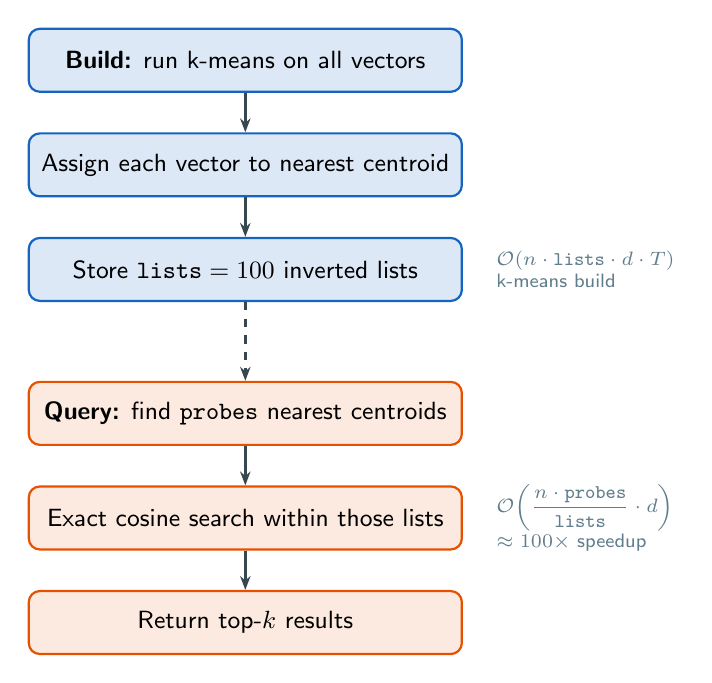
\begin{tikzpicture}[
  phase/.style={rectangle, rounded corners=4pt, minimum width=5.5cm,
                minimum height=0.8cm, text centered,
                font=\small\sffamily, draw, line width=0.8pt},
  arr/.style={-{Stealth[length=5pt]}, darkgray, line width=0.9pt},
  node distance=0.5cm,
]
  \node[phase, fill=nodeblue!15, draw=nodeblue]     (b1) {\textbf{Build:} run k-means on all vectors};
  \node[phase, fill=nodeblue!15, draw=nodeblue, below=of b1] (b2) {Assign each vector to nearest centroid};
  \node[phase, fill=nodeblue!15, draw=nodeblue, below=of b2] (b3) {Store $\texttt{lists}=100$ inverted lists};

  \node[phase, fill=nodeorange!12, draw=nodeorange, below=1cm of b3] (q1) {\textbf{Query:} find \texttt{probes} nearest centroids};
  \node[phase, fill=nodeorange!12, draw=nodeorange, below=of q1]     (q2) {Exact cosine search within those lists};
  \node[phase, fill=nodeorange!12, draw=nodeorange, below=of q2]     (q3) {Return top-$k$ results};

  \draw[arr] (b1)--(b2); \draw[arr] (b2)--(b3);
  \draw[arr,dashed] (b3) -- ++(0,-0.5) -- (q1);
  \draw[arr] (q1)--(q2); \draw[arr] (q2)--(q3);

  \node[right=0.3cm of b3, font=\scriptsize\sffamily\color{medgray}, align=left]
    {$\mathcal{O}(n \cdot \texttt{lists} \cdot d \cdot T)$\\k-means build};
  \node[right=0.3cm of q2, font=\scriptsize\sffamily\color{medgray}, align=left]
    {$\mathcal{O}\!\left(\dfrac{n\cdot\texttt{probes}}{\texttt{lists}}\cdot d\right)$\\$\approx 100\times$ speedup};
\end{tikzpicture}
\caption{IVFFlat build and query phases.  With \texttt{lists=100} and
  \texttt{probes=1}, each query scans $\approx 1\%$ of vectors.}
\end{figure}

\subsection{Confidence Scoring Model}

Confidence $c \in [0,1]$ is assigned by the LLM per claim following an explicit
rubric in the system prompt:

\begin{table}[H]
\centering\small
\begin{tabularx}{\linewidth}{C{2.0cm} L{4.0cm} X}
\toprule
\rowcolor{headerrow}
\color{white}\textbf{Range} & \color{white}\textbf{Interpretation} & \color{white}\textbf{Example} \\
\midrule
$[0.9,\,1.0]$ & Explicitly stated fact & ``I am the VP of Trading'' \\
\rowcolor{rowalt}
$[0.7,\,0.8]$ & Strongly implied        & ``As we discussed in our team meeting'' \\
$[0.5,\,0.6]$ & Weakly implied          & Contextual inference \\
\rowcolor{rowalt}
$<0.4$        & \textbf{Filtered out}   & Below \code{extraction\_min\_confidence} \\
\bottomrule
\end{tabularx}
\caption{Confidence rubric enforced in the LLM system prompt.}
\end{table}

\subsection{Extraction Versioning \& Idempotency}

The version tag is a deterministic fingerprint:
\begin{equation}
  v = \underbrace{\texttt{v1.0}}_{\text{schema}}
    \mathbin{\|} \underbrace{\texttt{model\_name}}_{\text{e.g., llama-3.3-70b}}
    \mathbin{\|} \underbrace{\mathrm{SHA\text{-}256}(\texttt{SYSTEM\_PROMPT})[:8]}_{\text{prompt hash}}
\end{equation}

Idempotency is enforced at the database level:
\begin{lstlisting}[language=SQL, caption={Idempotent unprocessed email query}]
SELECT r.*
FROM   raw_emails r
LEFT   JOIN processing_log p
         ON r.message_id = p.email_id
        AND p.extraction_version = :version
WHERE  p.id IS NULL
LIMIT  :batch_size;
\end{lstlisting}

Any change to \{prompt, model, schema\} generates a new tag, causing all emails
to be reprocessed while old extraction records are preserved.

% ══════════════════════════════════════════════════════════════════════════════
\section{Pipeline Orchestration \& Temporal Model}
% ══════════════════════════════════════════════════════════════════════════════

\subsection{Three-Stage Orchestrator (\code{pipeline.py})}

\begin{figure}[H]
\centering
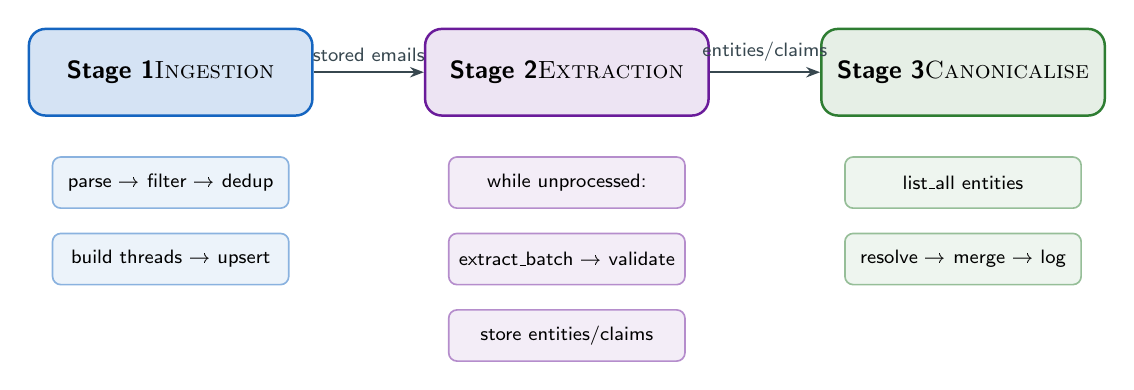
\begin{tikzpicture}[
  stage/.style={rectangle, rounded corners=6pt, minimum width=3.6cm,
                minimum height=1.1cm, text centered,
                font=\small\sffamily, draw, line width=0.9pt},
  sub/.style={rectangle, rounded corners=3pt, minimum width=3.0cm,
              minimum height=0.65cm, text centered,
              font=\scriptsize\sffamily, draw, line width=0.6pt},
  arr/.style={-{Stealth[length=5pt]}, darkgray, line width=0.9pt},
  node distance=0.5cm and 1.6cm,
]
  \node[stage, fill=nodeblue!18, draw=nodeblue] (s1) {\textbf{Stage 1}\\\textsc{Ingestion}};
  \node[stage, fill=nodepurple!12, draw=nodepurple, right=1.4cm of s1] (s2) {\textbf{Stage 2}\\\textsc{Extraction}};
  \node[stage, fill=nodegreen!12, draw=nodegreen, right=1.4cm of s2] (s3) {\textbf{Stage 3}\\\textsc{Canonicalise}};

  \draw[arr] (s1)--(s2) node[midway, above, font=\scriptsize\sffamily]{stored emails};
  \draw[arr] (s2)--(s3) node[midway, above, font=\scriptsize\sffamily]{entities/claims};

  % sub-bullets
  \node[sub, fill=nodeblue!8, draw=nodeblue!50, below=0.5cm of s1, xshift=0] (s1a)
    {parse → filter → dedup};
  \node[sub, fill=nodeblue!8, draw=nodeblue!50, below=0.3cm of s1a] (s1b)
    {build threads → upsert};

  \node[sub, fill=nodepurple!8, draw=nodepurple!50, below=0.5cm of s2] (s2a)
    {while unprocessed:};
  \node[sub, fill=nodepurple!8, draw=nodepurple!50, below=0.3cm of s2a] (s2b)
    {extract\_batch → validate};
  \node[sub, fill=nodepurple!8, draw=nodepurple!50, below=0.3cm of s2b] (s2c)
    {store entities/claims};

  \node[sub, fill=nodegreen!8, draw=nodegreen!50, below=0.5cm of s3] (s3a)
    {list\_all entities};
  \node[sub, fill=nodegreen!8, draw=nodegreen!50, below=0.3cm of s3a] (s3b)
    {resolve → merge → log};
\end{tikzpicture}
\caption{Three-stage pipeline orchestrator.  Each stage is independently
  resumable.  Errors in one email do not stop the batch.}
\end{figure}

\subsection{Bitemporal Claim Model}

Three independent time dimensions are maintained on every claim:

\begin{table}[H]
\centering\small
\begin{tabularx}{\linewidth}{L{2.8cm} L{3.0cm} X}
\toprule
\rowcolor{headerrow}
\color{white}\textbf{Dimension} & \color{white}\textbf{Column} & \color{white}\textbf{Meaning} \\
\midrule
Event time      & \code{valid\_from}    & When the real-world event occurred \\
\rowcolor{rowalt}
Validity time   & \code{valid\_to}      & When the claim ceased to be true (NULL = still valid) \\
Extraction time & \code{evidence.created\_at} & When our system extracted the claim \\
\bottomrule
\end{tabularx}
\end{table}

Role-change handling — \emph{no data is ever deleted}:
\begin{align*}
  &\text{Old:}\quad \textsc{works\_at}(\text{Skilling, Enron})
    \;[\,\text{valid\_from}=1997,\;\text{valid\_to}=2001\text{-}08\text{-}14,\;\text{is\_current}=\text{false}\,] \\
  &\text{New:}\quad \textsc{works\_at}(\text{Skilling, Enron})
    \;[\,\text{valid\_from}=2001\text{-}08\text{-}14,\;\text{valid\_to}=\text{NULL},\;\text{is\_current}=\text{true}\,]
\end{align*}

% ══════════════════════════════════════════════════════════════════════════════
\section{Quality Control}
% ══════════════════════════════════════════════════════════════════════════════

\begin{table}[H]
\centering\small
\begin{tabularx}{\linewidth}{L{3.6cm} X C{2.8cm}}
\toprule
\rowcolor{headerrow}
\color{white}\textbf{Metric} & \color{white}\textbf{Definition} & \color{white}\textbf{Target} \\
\midrule
Evidence verif.\ rate & \% of claims where excerpt is found in source & $> 95\%$ \\
\rowcolor{rowalt}
Entity resolution prec.\ & Manual audit: correct merges / total merges & $> 90\%$ \\
Confidence calibration & $|\,\overline{\text{acc}}_{c=0.9} - 0.9\,|$ & $\leq 5\%$ \\
\rowcolor{rowalt}
Extraction success rate & Successful LLM parses / total attempts & $> 85\%$ \\
\bottomrule
\end{tabularx}
\caption{Quality metrics and targets.  All drops are logged as
  \code{ValidationEvent} records for audit.}
\end{table}

% ══════════════════════════════════════════════════════════════════════════════
\section{Technology Stack}
% ══════════════════════════════════════════════════════════════════════════════

\begin{table}[H]
\centering\small
\begin{tabularx}{\linewidth}{L{3.0cm} L{3.8cm} X}
\toprule
\rowcolor{headerrow}
\color{white}\textbf{Category} & \color{white}\textbf{Technology} & \color{white}\textbf{Notes} \\
\midrule
Language        & Python 3.13          & Fully async (\code{asyncio} throughout) \\
\rowcolor{rowalt}
Schema valid.   & Pydantic v2          & Strict types, field/model validators \\
DB driver       & SQLAlchemy 2 + asyncpg & Async sessions, connection pooling \\
\rowcolor{rowalt}
Database        & PostgreSQL 16        & \code{pgvector}, \code{pg\_trgm}, \code{uuid-ossp} \\
Vector search   & pgvector             & IVFFlat index, cosine distance \\
\rowcolor{rowalt}
LLM (primary)   & Groq \code{llama-3.3-70b} & 80 RPM free-tier, JSON mode \\
LLM (fallback)  & Gemini \code{gemini-2.0-flash} & OpenAI-compatible endpoint \\
\rowcolor{rowalt}
Embeddings      & \code{all-MiniLM-L6-v2} & sentence-transformers, 384-dim \\
Fuzzy matching  & rapidfuzz            & Levenshtein ratio, partial\_ratio \\
\rowcolor{rowalt}
Near-dedup      & datasketch           & MinHash LSH, Jaccard similarity \\
Rate limiting   & aiolimiter           & Async token bucket \\
\rowcolor{rowalt}
Retry logic     & tenacity             & Exponential backoff \\
API framework   & FastAPI              & Async, Pydantic response models \\
\rowcolor{rowalt}
Frontend        & React + Vite + TS    & \code{webui/} directory \\
Logging         & structlog            & Structured JSON output \\
\rowcolor{rowalt}
Config          & pydantic-settings    & \code{.env} + env vars, \code{lru\_cache} \\
Containerised   & Docker Compose       & PostgreSQL + app service \\
\bottomrule
\end{tabularx}
\caption{Full technology stack.}
\end{table}

% ══════════════════════════════════════════════════════════════════════════════
\section{Scalability \& Production Roadmap}
% ══════════════════════════════════════════════════════════════════════════════

\begin{table}[H]
\centering\small
\begin{tabularx}{\linewidth}{L{3.0cm} L{3.8cm} X}
\toprule
\rowcolor{headerrow}
\color{white}\textbf{Aspect} & \color{white}\textbf{Current (Prototype)} & \color{white}\textbf{Production Target} \\
\midrule
Input scale     & $\sim$500K emails, 10 users & Millions of artefacts (email + Slack + Jira + Docs) \\
\rowcolor{rowalt}
Ingestion mode  & Batch file parsing (\code{iter\_maildir}) & Event-driven: Kafka/SQS → extract → store \\
LLM strategy    & Free-tier Groq / Gemini & Fine-tuned small model + large model for disambiguation \\
\rowcolor{rowalt}
Vector index    & IVFFlat (\code{pgvector}) & HNSW (higher recall) or Pinecone/Weaviate \\
Multi-tenancy   & Single workspace & Workspace-scoped RLS policies \\
\rowcolor{rowalt}
Identity resol. & Email address + name & + Slack handles + Jira usernames + SSO \\
Deletions       & Soft-delete only & GDPR: hard-delete evidence, cascade claims \\
\rowcolor{rowalt}
Observability   & Structured logs (stdout) & Datadog/Grafana: latency, quality, cost dashboards \\
Evaluation      & Manual audit         & CI/CD golden-set F1 regression \\
\rowcolor{rowalt}
Entity types    & 6 types, 9 claim types & + Ticket, Sprint, Decision, Action Item, Channel \\
\bottomrule
\end{tabularx}
\caption{Prototype vs.\ production comparison across key dimensions.}
\end{table}

\subsection*{Key Architectural Changes for Production}

\begin{enumerate}[leftmargin=*, itemsep=4pt]
  \item \textbf{Streaming ingestion:} Replace \code{iter\_maildir} with an
    event consumer.  Each new artefact triggers an individual extraction job,
    enabling near-real-time graph updates.
  \item \textbf{HNSW indexing:} Replace IVFFlat with HNSW for better recall
    at high query throughput (IVFFlat recall degrades with \code{probes=1}
    at large scale).
  \item \textbf{Extraction cost optimisation:} Route simple extraction tasks to
    a fine-tuned small model; use large frontier models only for ambiguous
    disambiguation.
  \item \textbf{Multi-tenant isolation:} Add \code{workspace\_id} foreign keys
    and PostgreSQL RLS policies to isolate tenant data at the query level.
  \item \textbf{Automated evaluation:} Maintain a golden extraction set;
    run F1 precision/recall checks in CI/CD to catch prompt or schema
    regressions before deployment.
\end{enumerate}

% ─── End ─────────────────────────────────────────────────────────────────────
\vfill
\begin{center}
\small\sffamily\color{medgray}
Layer10 Memory Graph — Architecture Report \quad|\quad March 6, 2026 \quad|\quad
\textit{Generated from source: \texttt{layer10-takehome/}}
\end{center}

\end{document}
